% Created 2019-01-14 Mon 09:59
% Intended LaTeX compiler: pdflatex
\documentclass[11pt]{article}
\usepackage[utf8]{inputenc}
\usepackage[T1]{fontenc}
\usepackage{graphicx}
\usepackage{grffile}
\usepackage{longtable}
\usepackage{wrapfig}
\usepackage{rotating}
\usepackage[normalem]{ulem}
\usepackage{amsmath}
\usepackage{textcomp}
\usepackage{amssymb}
\usepackage{capt-of}
\usepackage{hyperref}
\usepackage{color}
\usepackage{minted}
\usepackage{color}
\usepackage{minted}
\usepackage{parskip}
\usepackage{geometry}
\geometry{left=2.5cm,right=2.5cm,top=2.5cm,bottom=2.5cm}
\usepackage{graphicx}
\usepackage{subcaption}
\author{Daniel Moreno Manzano}
\date{\today}
\title{Simulation Results steps}
\hypersetup{
 pdfauthor={Daniel Moreno Manzano},
 pdftitle={Simulation Results steps},
 pdfkeywords={},
 pdfsubject={},
 pdfcreator={Emacs 25.1.1 (Org mode 9.1.14)}, 
 pdflang={English}}
\begin{document}

\maketitle


\section{Simplest benchmarks results}
\label{sec:org25b9f04}

\begin{table}[!htpb]
\caption{\label{tab:org1f4383c}
Benchmarks used}
\centering
\begin{tabular}{lrr}
\hline
Benchmark & \# qubits & \# gates\\
\hline
4gt11\(_{\text{82}}\) & 5 & 27\\
4gt12\(_{\text{v1}}\)\(_{\text{89}}\) & 6 & 228\\
4gt4\(_{\text{v0}}\)\(_{\text{72}}\) & 6 & 258\\
4mod5\(_{\text{bdd}}\)\(_{\text{287}}\) & 7 & 70\\
4mod5\(_{\text{v0}}\)\(_{\text{20}}\) & 5 & 20\\
alu\(_{\text{bdd}}\)\(_{\text{288}}\) & 7 & 84\\
alu\(_{\text{v0}}\)\(_{\text{27}}\) & 5 & 36\\
decod24\(_{\text{bdd}}\)\(_{\text{294}}\) & 6 & 73\\
decod24\(_{\text{enable}}\)\(_{\text{126}}\) & 6 & 338\\
graycode6\(_{\text{47}}\) & 6 & 5\\
ham3\(_{\text{102}}\) & 3 & 20\\
hwb4\(_{\text{49}}\) & 5 & 233\\
mod10\(_{\text{176}}\) & 5 & 178\\
mod5adder\(_{\text{127}}\) & 6 & 555\\
mod5d1\(_{\text{63}}\) & 5 & 22\\
mod8\(_{\text{10}}\)\(_{\text{177}}\) & 6 & 440\\
one\(_{\text{two}}\)\(_{\text{three}}\)\(_{\text{v1}}\)\(_{\text{99}}\) & 5 & 132\\
one\(_{\text{two}}\)\(_{\text{three}}\)\(_{\text{v3}}\)\(_{\text{101}}\) & 5 & 70\\
rd32\(_{\text{v0}}\)\(_{\text{66}}\) & 4 & 34\\
sf\(_{\text{274}}\) & 6 & 781\\
sf\(_{\text{276}}\) & 6 & 778\\
sym6\(_{\text{145}}\) & 7 & 3888\\
xor5\(_{\text{254}}\) & 6 & 7\\
\hline
\end{tabular}
\end{table}


\subsection{4gt11\(_{\text{82}}\)}
\label{sec:org4de07a2}

\begin{table}[H]
\caption{\label{tab:orgbc724f6}
Step 1 results after 1000 iterations}
\centering
\small
\begin{tabular}{lrrllrrr}
\hline
Mapper & \# qubits & depth & \# gates & \# SWAPS & p. success & \(f\) & \(V_Q\)\\
\hline
No & 5 & 78 & 84 & 0 & 0.96 & 0.97823066 & 390\\
\hline
minextendrc & 7 & 226 & 237 & 17 & 0.929 & 0.92937318 & 1582\\
minextend & 8 & \textbf{158} & \textbf{228} & \textbf{16} & \textbf{0.947} & \textbf{0.9312172} & 1264\\
base & 6 & 177 & \textbf{228} & \textbf{16} & 0.932 & 0.906571 & 1062\\
\hline
\end{tabular}
\end{table}

\subsection{4gt12-v1\(_{\text{89}}\)}
\label{sec:org7e3ffe8}

\begin{table}[H]
\caption{\label{tab:orgeb23346}
Results after 1000 iterations}
\centering
\small
\begin{tabular}{lrrrrrrr}
\hline
Mapper & \# qubits & depth & \# gates & \# SWAPS & p. success & \(f\) & \(V_Q\)\\
\hline
no & 6 & 416 & 658 & 0 & 0.768 & 0.66623522 & 2496\\
\hline
minextendrc & 9 & 1172 & \textbf{1360} & \textbf{78} & 0.562 & \textbf{0.44841106} & 10548\\
minextend & 9 & \textbf{1008} & 1549 & 99 & \textbf{0.601} & 0.40972458 & 9072\\
base & 6 & 1069 & 1423 & 85 & 0.517 & 0.3581228 & 6414\\
\hline
\end{tabular}
\end{table}


\subsection{4gt4-v0\(_{\text{72}}\)}
\label{sec:org1103a7f}

\begin{table}[H]
\caption{\label{tab:orgd091311}
Results after 1000 iterations}
\centering
\small
\begin{tabular}{lrrrrrrr}
\hline
Mapper & \# qubits & depth & \# gates & \# SWAPS & p. success & \(f\) & \(V_Q\)\\
\hline
no & 6 & 442 & 746 & 0 & 0.786 & 0.68007548 & 2652\\
\hline
minextendrc & 9 & 1352 & 1592 & 94 & 0.452 & \textbf{0.37749204} & 12168\\
minextend & 8 & \textbf{963} & 1736 & 110 & 0.498 & 0.34067243 & 7704\\
base & 6 & 1056 & \textbf{1547} & \textbf{89} & \textbf{0.532} & 0.35703954 & 6336\\
\hline
\end{tabular}
\end{table}

\subsection{4mod5-bdd\(_{\text{287}}\)}
\label{sec:org5759ff3}
\begin{table}[H]
\caption{\label{tab:org1043191}
Results after 1000 iterations}
\centering
\small
\begin{tabular}{lrrrrrrr}
\hline
Mapper & \# qubits & depth & \# gates & \# SWAPS & p. success & \(f\) & \(V_Q\)\\
\hline
no & 7 & 147 & 203 & 0 & 0.916 & 0.87474237 & 1029\\
\hline
minextendrc & 9 & 436 & 500 & 33 & 0.753 & 0.65935538 & 3924\\
minextend & 9 & \textbf{332} & 500 & 33 & \textbf{0.798} & \textbf{0.69281491} & 2988\\
base & 7 & 334 & \textbf{419} & \textbf{24} & 0.776 & 0.67942877 & 2338\\
\hline
\end{tabular}
\end{table}


\subsection{4mod5-v0\(_{\text{20}}\)}
\label{sec:org46dd7c7}
\begin{table}[H]
\caption{\label{tab:org92b9b48}
Results after 1000 iterations}
\centering
\small
\begin{tabular}{lrrrrrrr}
\hline
Mapper & \# qubits & depth & \# gates & \# SWAPS & p. success & \(f\) & \(V_Q\)\\
\hline
no & 5 & 53 & 61 & 0 & 0.985 & 0.97145968 & 265\\
\hline
minextendrc & 9 & 139 & 142 & 9 & 0.944 & \textbf{0.9092329} & 1251\\
minextend & 8 & \textbf{128} & 160 & 11 & 0.938 & 0.88981602 & 1024\\
base & 6 & 133 & \textbf{119} & \textbf{8} & \textbf{0.947} & 0.89871898 & 714\\
\hline
\end{tabular}
\end{table}

\subsection{alu\(_{\text{bdd}}\)\(_{\text{288}}\)}
\label{sec:org621e3f6}

\begin{table}[H]
\caption{\label{tab:orga9d546a}
Results after 1000 iterations}
\centering
\small
\begin{tabular}{lrrrrrrr}
\hline
Mapper & \# qubits & \# gates & \# SWAPS & depth & p. success & \(f\) & \(V_Q\)\\
\hline
no & 7 & 247 & 0 & 165 & 0.94 & 0.89851036 & 1155\\
\hline
minextendrc & 8 & 571 & 36 & 495 & \textbf{0.847} & \textbf{0.78096707} & 3960\\
minextend & 8 & 616 & 41 & 383 & 0.846 & 0.73109047 & 3064\\
base & 7 & \textbf{472} & \textbf{25} & \textbf{360} & 0.841 & 0.71637503 & 2520\\
\hline
\end{tabular}
\end{table}
\subsection{alu\(_{\text{v0}}\)\(_{\text{27}}\)}
\label{sec:org42ae2a6}
\begin{table}[H]
\caption{\label{tab:orgf9b02e3}
Results after 1000 iterations}
\centering
\small
\begin{tabular}{lrllrrrr}
\hline
Mapper & \# qubits & \# gates & \# SWAPS & depth & p. success & \(f\) & \(V_Q\)\\
\hline
no & 5 & 107 & 0 & 80 & 0.98 & 0.96369032 & 400\\
\hline
minextendrc & 9 & \textbf{278} & \textbf{19} & 248 & \textbf{0.959} & \textbf{0.92602273} & 2232\\
minextend & 10 & 296 & 21 & \textbf{156} & 0.944 & 0.89032214 & 1560\\
base & 6 & \textbf{278} & \textbf{19} & 214 & 0.915 & 0.84492332 & 1284\\
\hline
\end{tabular}
\end{table}
\subsection{decod24\(_{\text{bdd}}\)\(_{\text{294}}\)}
\label{sec:org71a319f}
\begin{table}[H]
\caption{\label{tab:orgb7dcdd7}
Results after 1000 iterations}
\centering
\small
\begin{tabular}{lrrrrrrr}
\hline
Mapper & \# qubits & \# gates & \# SWAPS & depth & p. success & \(f\) & \(V_Q\)\\
\hline
no & 6 & 207 & 0 & 144 & 0.938 & 0.91098461 & 864\\
\hline
minextendrc & 9 & 441 & 26 & 407 & \textbf{0.888} & \textbf{0.7749599} & 3663\\
minextend & 7 & 468 & 29 & 328 & 0.816 & 0.73708015 & 2296\\
base & 6 & \textbf{405} & \textbf{22} & \textbf{300} & 0.781 & 0.71803687 & 1800\\
\hline
\end{tabular}
\end{table}
\subsection{decod24\(_{\text{enable}}\)\(_{\text{126}}\)}
\label{sec:org6a4f258}
\begin{table}[H]
\caption{\label{tab:org81f8517}
Results after 1000 iterations}
\centering
\small
\begin{tabular}{lrrrrrrr}
\hline
Mapper & \# qubits & \# gates & \# SWAPS & depth & p. success & \(f\) & \(V_Q\)\\
\hline
no & 6 & 978 & 0 & 612 & 0.894 & 0.74038417 & 3672\\
\hline
minextendrc & 9 & 2049 & 119 & 1788 & \textbf{0.831} & \textbf{0.57285276} & 16092\\
minextend & 10 & 2184 & 134 & \textbf{1440} & 0.805 & 0.50947313 & 14400\\
base & 6 & \textbf{1959} & \textbf{109} & 1446 & 0.74 & 0.42630108 & 8676\\
\hline
\end{tabular}
\end{table}
\subsection{graycode6\(_{\text{47}}\)}
\label{sec:org74d64b7}
\begin{table}[H]
\caption{\label{tab:orgaa45f1c}
Results after 1000 iterations}
\centering
\small
\begin{tabular}{lrrrrrrr}
\hline
Mapper & \# qubits & \# gates & \# SWAPS & depth & p. success & \(f\) & \(V_Q\)\\
\hline
no & 6 & 21 & 0 & 32 & 0.995 & 0.99332325 & 192\\
\hline
minextendrc & 7 & 111 & 10 & 111 & 0.991 & 0.98223938 & 777\\
minextend & 10 & 102 & 9 & 61 & 0.987 & 0.97012132 & 610\\
base & 6 & 84 & 7 & 82 & 0.991 & 0.98075312 & 492\\
\hline
\end{tabular}
\end{table}
\subsection{ham3\(_{\text{102}}\)}
\label{sec:org78aaaf3}
\begin{table}[H]
\caption{\label{tab:orgd48dfa4}
Results after 1000 iterations}
\centering
\small
\begin{tabular}{lrrrrrrr}
\hline
Mapper & \# qubits & \# gates & \# SWAPS & depth & p. success & \(f\) & \(V_Q\)\\
\hline
no & 3 & 61 & 0 & 60 & 0.987 & 0.98246387 & 180\\
\hline
minextendrc & 4 & 115 & 6 & 127 & 0.971 & 0.95999051 & 508\\
minextend & 4 & 115 & 6 & 121 & 0.974 & 0.96288976 & 484\\
base & 4 & 106 & 5 & 98 & 0.973 & 0.95944625 & 392\\
\hline
\end{tabular}
\end{table}
\subsection{mod10\(_{\text{176}}\)}
\label{sec:org7634139}
\begin{table}[H]
\caption{\label{tab:orgbb9e57f}
Results after 1000 iterations, \(t_1 = t_2 = 3000\)}
\centering
\small
\begin{tabular}{lrrrrrrr}
\hline
Mapper & \# qubits & \# gates & \# SWAPS & depth & p. success & \(f\) & \(V_Q\)\\
\hline
no & 5 & 515 & 0 & 327 & 0.9 & 0.82976826 & 1635\\
\hline
minextendrc & 7 & 1199 & 76 & 1090 & \textbf{0.758} & \textbf{0.62105388} & 7630\\
minextend & 10 & 1127 & 68 & \textbf{687} & 0.733 & 0.60641905 & 6870\\
base & 6 & \textbf{983} & \textbf{52} & 734 & 0.697 & 0.56115058 & 4404\\
\hline
\end{tabular}
\end{table}

\begin{table}[H]
\caption{\label{tab:org38cd1a9}
Results after 1000 iterations, \(t_1 = t_2 = 1000\)}
\centering
\small
\begin{tabular}{lrr}
\hline
Mapper & p. success & \(f\)\\
\hline
no & 0.738 & 0.59602509\\
\hline
minextendrc & \textbf{0.453} & \textbf{0.31989048}\\
minextend & 0.443 & 0.31320313\\
base & 0.372 & 0.27839542\\
\hline
\end{tabular}
\end{table}

\subsection{mod5adder\(_{\text{127}}\)}
\label{sec:org67c3e45}
\begin{table}[H]
\caption{\label{tab:orgd374d62}
Results after 1000 iterations, \(t_1 = t_2 = 3000\)}
\centering
\small
\begin{tabular}{lrrrrrrr}
\hline
Mapper & \# qubits & \# gates & \# SWAPS & depth & p. success & \(f\) & \(V_Q\)\\
\hline
no & 6 & 1583 & 0 & 944 & 0.71 & 0.45135226 & 5664\\
\hline
minextendrc & 9 & 3320 & 193 & 2878 & 0.491 & \textbf{0.1922222} & 25902\\
minextend & 10 & 3779 & 244 & 2667 & 0.548 & 0.18165444 & 26670\\
base & 6 & \textbf{3248} & \textbf{185} & \textbf{2378} & \textbf{0.591} & 0.18911191 & 14268\\
\hline
\end{tabular}
\end{table}

\begin{table}[H]
\caption{\label{tab:org3a5be80}
Results after 1000 iterations, \(t_1 = t_2 = 1000\)}
\centering
\small
\begin{tabular}{lrr}
\hline
Mapper & p. success & \(f\)\\
\hline
no & 0.528 & 0.18188697\\
\hline
minextendrc & 0.36 & \textbf{0.1484162}\\
minextend & 0.399 & 0.14349585\\
base & \textbf{0.465} & 0.12694018\\
\hline
\end{tabular}
\end{table}
\subsection{mod5d1\(_{\text{63}}\)}
\label{sec:org4c69f04}
\begin{table}[H]
\caption{\label{tab:orgcf0ed24}
Results after 1000 iterations, \(t_1 = t_2 = 3000\)}
\centering
\small
\begin{tabular}{lrllrrrr}
\hline
Mapper & \# qubits & \# gates & \# SWAPS & depth & p. success & \(f\) & \(V_Q\)\\
\hline
no & 5 & 69 & 0 & 59 & 0.989 & 0.98368741 & 295\\
\hline
minextendrc & 8 & \textbf{195} & \textbf{14} & 209 & 0.958 & 0.93474128 & 1672\\
minextend & 8 & \textbf{195} & \textbf{14} & \textbf{136} & \textbf{0.969} & \textbf{0.93997349} & 1088\\
base & 6 & \textbf{195} & \textbf{14} & 146 & 0.95 & 0.91002595 & 876\\
\hline
\end{tabular}
\end{table}

\begin{table}[H]
\caption{\label{tab:org449ea4e}
Results after 1000 iterations, \(t_1 = t_2 = 1000\)}
\centering
\small
\begin{tabular}{lrr}
\hline
Mapper & p. success & \(f\)\\
\hline
no & 0.97 & 0.95187372\\
\hline
minextendrc & 0.901 & \textbf{0.84099717}\\
minextend & \textbf{0.914} & 0.83627787\\
base & 0.892 & 0.7849484\\
\hline
\end{tabular}
\end{table}

\subsection{mod8\(_{\text{10}}\)\(_{\text{177}}\)}
\label{sec:org3b574a0}
\begin{table}[H]
\caption{\label{tab:orgfa001f3}
Results after 1000 iterations, \(t_1 = t_2 = 3000\)}
\centering
\small
\begin{tabular}{lrrrrrrr}
\hline
Mapper & \# qubits & \# gates & \# SWAPS & depth & p. success & \(f\) & \(V_Q\)\\
\hline
no & 6 & 1270 & 0 & 794 & 0.858 & 0.70131629 & 4764\\
\hline
minextendrc & 10 & \textbf{2674} & \textbf{156} & 2275 & \textbf{0.52} & \textbf{0.39211003} & 22750\\
minextend & 10 & 2827 & 173 & \textbf{1761} & 0.411 & 0.29686116 & 17610\\
base & 6 & 2773 & 167 & 2006 & 0.335 & 0.26106507 & 12036\\
\hline
\end{tabular}
\end{table}

\begin{table}[H]
\caption{\label{tab:orgf4a8058}
Results after 1000 iterations, \(t_1 = t_2 = 1000\)}
\centering
\small
\begin{tabular}{lrr}
\hline
Mapper & p. success & \(f\)\\
\hline
no & 0.698 & 0.42021822\\
\hline
minextendrc & 0.244 & 0.19792409\\
minextend & 0.123 & 0.14638911\\
base & 0.068 & 0.16412249\\
\hline
\end{tabular}
\end{table}
\subsection{one\(_{\text{two}}\)\(_{\text{three}}\)\(_{\text{v1}}\)\(_{\text{99}}\)}
\label{sec:org334eaae}
\begin{table}[H]
\caption{\label{tab:orga5b500d}
Results after 1000 iterations, \(t_1 = t_2 = 3000\)}
\centering
\small
\begin{tabular}{lrrrrrrr}
\hline
Mapper & \# qubits & \# gates & \# SWAPS & depth & p. success & \(f\) & \(V_Q\)\\
\hline
no & 5 & 383 & 0 & 256 & 0.832 & 0.78653106 & 1280\\
\hline
minextendrc & 7 & 887 & 56 & 839 & 0.633 & 0.59855522 & 5873\\
minextend & 10 & 869 & 54 & \textbf{530} & \textbf{0.729} & \textbf{0.62135956} & 5300\\
base & 6 & \textbf{833} & \textbf{50} & 609 & 0.662 & 0.57083541 & 3654\\
\hline
\end{tabular}
\end{table}

\begin{table}[H]
\caption{\label{tab:org8885bcf}
Results after 1000 iterations, \(t_1 = t_2 = 1000\)}
\centering
\small
\begin{tabular}{lrr}
\hline
Mapper & p. success & \(f\)\\
\hline
no & 0.602 & 0.55524768\\
\hline
minextendrc & 0.266 & \textbf{0.38317882}\\
minextend & \textbf{0.355} & 0.33820922\\
base & 0.26 & 0.31493265\\
\hline
\end{tabular}
\end{table}
\subsection{one\(_{\text{two}}\)\(_{\text{three}}\)\(_{\text{v3}}\)\(_{\text{101}}\)}
\label{sec:orgd62faff}
\begin{table}[H]
\caption{\label{tab:org7745fc3}
Results after 1000 iterations, \(t_1 = t_2 = 3000\)}
\centering
\small
\begin{tabular}{lrrrrrrr}
\hline
Mapper & \# qubits & \# gates & \# SWAPS & depth & p. success & \(f\) & \(V_Q\)\\
\hline
no & 5 & 203 & 0 & 143 & 0.937 & 0.88807716 & 715\\
\hline
minextendrc & 8 & 464 & 29 & 440 & \textbf{0.746} & 0.620299 & 3520\\
minextend & 8 & 509 & 34 & \textbf{302} & 0.732 & 0.63161506 & 2416\\
base & 6 & \textbf{428} & \textbf{25} & 323 & 0.742 & \textbf{0.62081173} & 1938\\
\hline
\end{tabular}
\end{table}

\begin{table}[H]
\caption{\label{tab:org1c6020d}
Results after 1000 iterations, \(t_1 = t_2 = 1000\)}
\centering
\small
\begin{tabular}{lrr}
\hline
Mapper & p. success & \(f\)\\
\hline
no & 0.809 & 0.69629912\\
\hline
minextendrc & 0.411 & 0.31374806\\
minextend & 0.391 & \textbf{0.31579028}\\
base & \textbf{0.42} & 0.31189591\\
\hline
\end{tabular}
\end{table}
\subsection{rd32\(_{\text{v0}}\)\(_{\text{66}}\)}
\label{sec:org13453d3}
\begin{table}[H]
\caption{\label{tab:org65b6b57}
Results after 1000 iterations, \(t_1 = t_2 = 3000\)}
\centering
\small
\begin{tabular}{lrllrrrr}
\hline
Mapper & \# qubits & \# gates & \# SWAPS & depth & p. success & \(f\) & \(V_Q\)\\
\hline
no & 4 & 102 & 0 & 83 & 0.983 & 0.97241164 & 332\\
\hline
minextendrc & 7 & \textbf{219} & \textbf{13} & 195 & 0.947 & \textbf{0.91458844} & 1365\\
minextend & 7 & 228 & 14 & \textbf{142} & \textbf{0.958} & 0.91079208 & 994\\
base & 5 & \textbf{219} & \textbf{13} & 169 & 0.955 & 0.90759692 & 845\\
\hline
\end{tabular}
\end{table}

\begin{table}[H]
\caption{\label{tab:org39c71e1}
Results after 1000 iterations, \(t_1 = t_2 = 1000\)}
\centering
\small
\begin{tabular}{lrr}
\hline
Mapper & p. success & \(f\)\\
\hline
no & 0.95 & 0.9176419\\
\hline
minextendrc & 0.88 & \textbf{0.79475368}\\
minextend & \textbf{0.902} & 0.77708902\\
base & 0.896 & 0.77242986\\
\hline
\end{tabular}
\end{table}
\subsection{sf\(_{\text{274}}\)}
\label{sec:org72bdf2a}
\begin{table}[H]
\caption{\label{tab:org215695a}
Results after 1000 iterations, \(t_1 = t_2 = 3000\)}
\centering
\small
\begin{tabular}{lrrrrrrr}
\hline
Mapper & \# qubits & \# gates & \# SWAPS & depth & p. success & \(f\) & \(V_Q\)\\
\hline
no & 6 & 2227 & 0 & 1359 & 0.484 & 0.34974095 & 8154\\
\hline
minextendrc & 7 & 5116 & 321 & 4515 & 0.0 & \textbf{0.16778098} & 31605\\
minextend & 10 & 5071 & 316 & \textbf{3007} & \textbf{0.097} & 0.14752778 & 30070\\
base & 6 & \textbf{4450} & \textbf{247} & 3289 & 0.088 & 0.15461728 & 19734\\
\hline
\end{tabular}
\end{table}

\begin{table}[H]
\caption{\label{tab:org2051682}
Results after 1000 iterations, \(t_1 = t_2 = 1000\)}
\centering
\small
\begin{tabular}{lrr}
\hline
Mapper & p. success & \(f\)\\
\hline
no & 0.108 & 0.16219308\\
\hline
minextendrc & \textbf{0.002} & \textbf{0.19857107}\\
minextend & 0.0 & 0.1458942\\
base & 0.0 & 0.14493197\\
\hline
\end{tabular}
\end{table}
\subsection{sf\(_{\text{276}}\)}
\label{sec:org00e6e35}
\begin{table}[H]
\caption{\label{tab:org9d5e6c4}
Results after 1000 iterations, \(t_1 = t_2 = 3000\)}
\centering
\small
\begin{tabular}{lrrrrrrr}
\hline
Mapper & \# qubits & \# gates & \# SWAPS & depth & p. success & \(f\) & \(V_Q\)\\
\hline
no & 6 & 2224 & 0 & 1360 & 0.472 & 0.30846996 & 8160\\
\hline
minextendrc & 9 & 4852 & 292 & 4103 & 0.0 & \textbf{0.16746873} & 36927\\
minextend & 10 & 4807 & 287 & \textbf{2747} & \textbf{0.092} & 0.14342305 & 27470\\
base & 6 & \textbf{4447} & \textbf{247} & 3280 & 0.089 & 0.13928494 & 19680\\
\hline
\end{tabular}
\end{table}

\begin{table}[H]
\caption{\label{tab:orgc8685aa}
Results after 1000 iterations, \(t_1 = t_2 = 1000\)}
\centering
\small
\begin{tabular}{lrr}
\hline
Mapper & p. success & \(f\)\\
\hline
no & 0.034 & 0.15718296\\
\hline
minextendrc & 0.0 & \textbf{0.22111901}\\
minextend & 0.0 & 0.15992956\\
base & 0.0 & 0.14842314\\
\hline
\end{tabular}
\end{table}
\subsection{sym6\(_{\text{145}}\)}
\label{sec:org72c936a}
\begin{table}[H]
\caption{\label{tab:org5e55677}
Results after 1000 iterations, \(t_1 = t_2 = 3000\)}
\centering
\small
\begin{tabular}{lrrrrrrr}
\hline
Mapper & \# qubits & \# gates & \# SWAPS & depth & p. success & \(f\) & \(V_Q\)\\
\hline
no & 7 & 11185 & 0 & 6759 & 0.506 & 0.15429107 & 47313\\
\hline
minextendrc & 8 & 24658 & 1497 & 20984 & 0.513 & \textbf{0.22079977} & 167872\\
minextend & 10 & 25756 & 1619 & \textbf{14156} & \textbf{0.546} & 0.12489321 & 141560\\
base & 7 & \textbf{21679} & \textbf{1166} & 15613 & 0.531 & 0.12176519 & 109291\\
\hline
\end{tabular}
\end{table}

\begin{table}[H]
\caption{\label{tab:orgf915b0a}
Results after 1000 iterations, \(t_1 = t_2 = 1000\)}
\centering
\small
\begin{tabular}{lrr}
\hline
Mapper & p. success & \(f\)\\
\hline
no & 0.513 & 0.1407412\\
\hline
minextendrc & 0.518 & \textbf{0.24438143}\\
minextend & \textbf{0.543} & 0.1533595\\
base & 0.53 & 0.14274046\\
\hline
\end{tabular}
\end{table}

\subsection{xor5\(_{\text{254}}\)}
\label{sec:orgc175172}
\begin{table}[H]
\caption{\label{tab:org0bf421b}
Results after 1000 iterations, \(t_1 = t_2 = 3000\)}
\centering
\small
\begin{tabular}{lrrrrrrr}
\hline
Mapper & \# qubits & \# gates & \# SWAPS & depth & p. success & \(f\) & \(V_Q\)\\
\hline
no & 6 & 23 & 0 & 36 & 0.995 & 0.99375935 & 216\\
\hline
minextendrc & 7 & 68 & 5 & 75 & 0.984 & 0.9736118 & 525\\
minextend & 7 & 68 & 5 & 58 & 0.958 & 0.94092446 & 406\\
base & 6 & 104 & 9 & 92 & 0.942 & 0.91559086 & 552\\
\hline
\end{tabular}
\end{table}

\begin{table}[H]
\caption{\label{tab:org212d364}
Results after 1000 iterations, \(t_1 = t_2 = 3000\)}
\centering
\small
\begin{tabular}{lrr}
\hline
Mapper & p. success & \(f\)\\
\hline
no & 0.984 & 0.97720823\\
\hline
minextendrc & \textbf{0.952} & \textbf{0.91998206}\\
minextend & 0.896 & 0.84674549\\
base & 0.837 & 0.77312906\\
\hline
\end{tabular}
\end{table}

\section{Correlation and Plots}
\label{sec:org4bd68a5}

Pearson correlation formula:

$${\displaystyle \rho _{X,Y}={\frac {\operatorname {cov} (X,Y)}{\sigma _{X}\sigma _{Y}}}}$$

\subsection{\(t_1=3000\)}
\label{sec:org3d29e2c}

\begin{center}
\captionof{table}{\label{tab:orgb1a4bd1}
Pearson correlation coefficient for decoherence time of \(t_1 = 3000\) and measurement error 0f 0.005}
\begin{tabular}{lrrrr}
 & \# of Gates & \# of SWAPs & Depth & \(V_Q\)\\
\hline
\(\rho _{f,Y}\) & -0.9360 & -0.8614 & -0.9091 & -0.8728\\
\(\rho _{p_s,Y}\) & -0.9257 & -0.8700 & -0.9060 & -0.8680\\
\hline
\end{tabular}
\end{center}

\begin{figure}[H] 
  \begin{subfigure}[b]{0.5\linewidth}
    \centering
    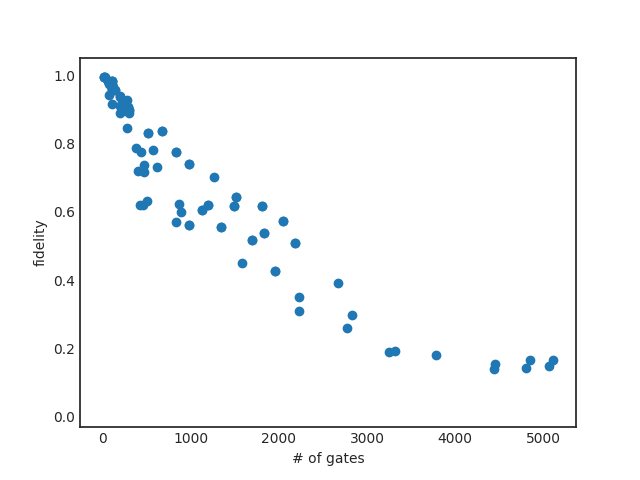
\includegraphics[width=0.75\linewidth]{f_g_3000_0_005} 
    \caption{Number of gates} 
    \label{fig:f_g_3000} 
    \vspace{4ex}
  \end{subfigure}%% 
  \begin{subfigure}[b]{0.5\linewidth}
    \centering
    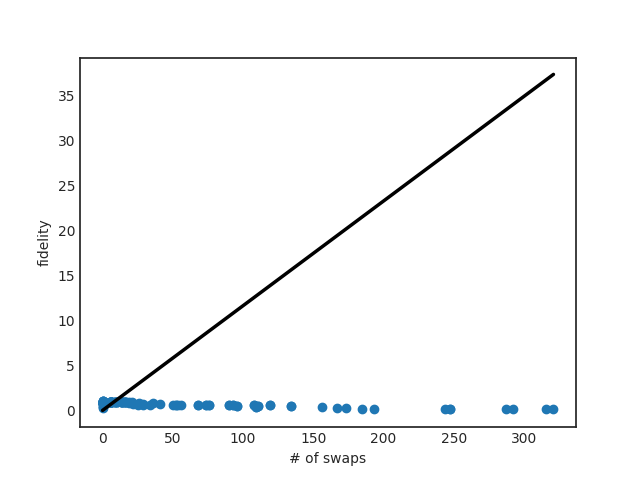
\includegraphics[width=0.75\linewidth]{f_s_3000_0_005} 
    \caption{Number of SWAPs} 
    \label{fig:f_s_3000} 
    \vspace{4ex}
  \end{subfigure} 
  \begin{subfigure}[b]{0.5\linewidth}
    \centering
    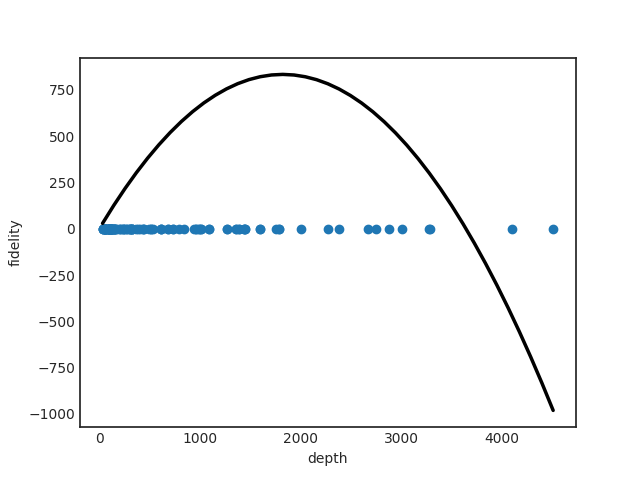
\includegraphics[width=0.75\linewidth]{f_d_3000_0_005} 
    \caption{Depth} 
    \label{fig:f_d_3000} 
  \end{subfigure}%%
  \begin{subfigure}[b]{0.5\linewidth}
    \centering
    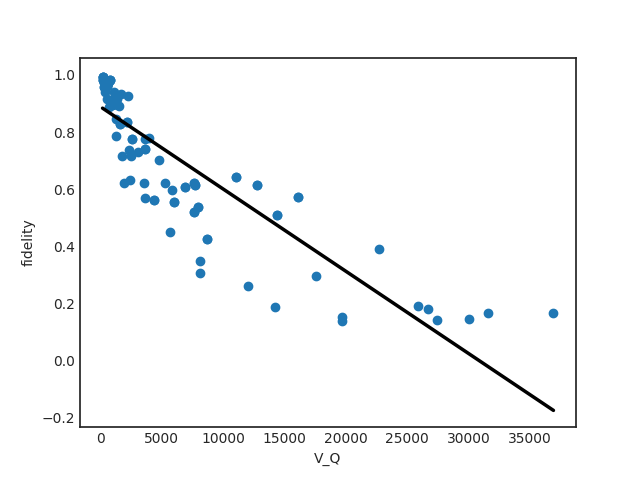
\includegraphics[width=0.75\linewidth]{f_q_3000_0_005} 
    \caption{Quantum Volume} 
    \label{fig:f_q_3000} 
  \end{subfigure} 
  \caption{Plotting fidelity against number of gates, swaps, depth and Quantum Volume}
  \label{fig:f_3000} 
\end{figure}

\begin{figure}[H] 
  \begin{subfigure}[b]{0.5\linewidth}
    \centering
    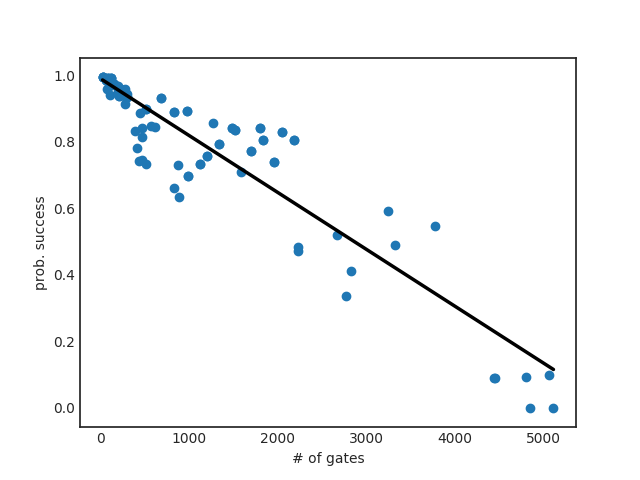
\includegraphics[width=0.75\linewidth]{ps_g_3000_0_005} 
    \caption{Number of gates} 
    \label{fig:ps_g_3000} 
    \vspace{4ex}
  \end{subfigure}%% 
  \begin{subfigure}[b]{0.5\linewidth}
    \centering
    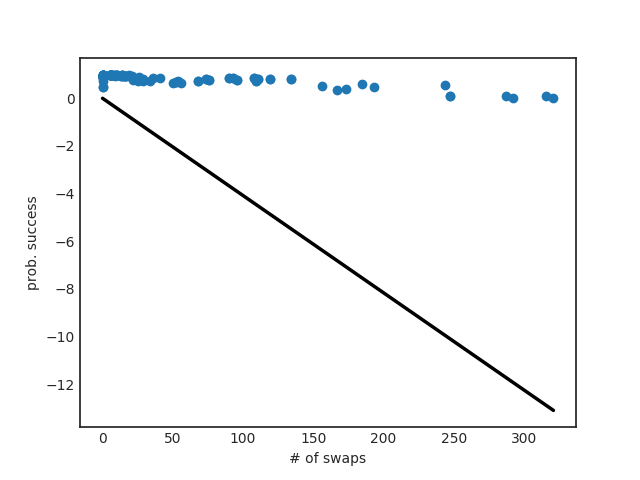
\includegraphics[width=0.75\linewidth]{ps_s_3000_0_005} 
    \caption{Number of SWAPs} 
    \label{fig:ps_s_3000} 
    \vspace{4ex}
  \end{subfigure} 
  \begin{subfigure}[b]{0.5\linewidth}
    \centering
    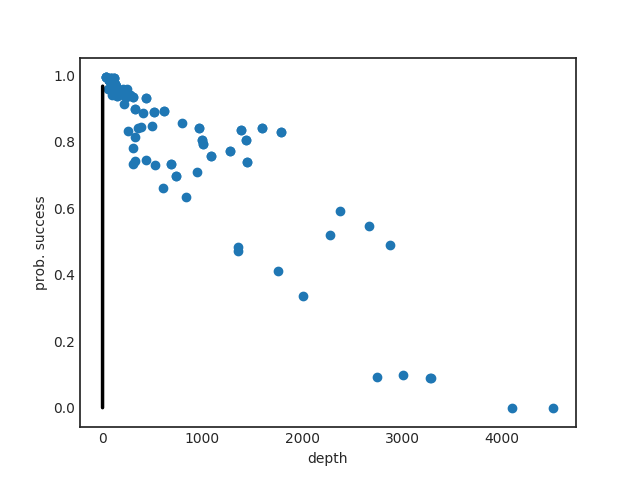
\includegraphics[width=0.75\linewidth]{ps_d_3000_0_005} 
    \caption{Depth} 
    \label{fig:ps_d_3000} 
  \end{subfigure}%%
  \begin{subfigure}[b]{0.5\linewidth}
    \centering
    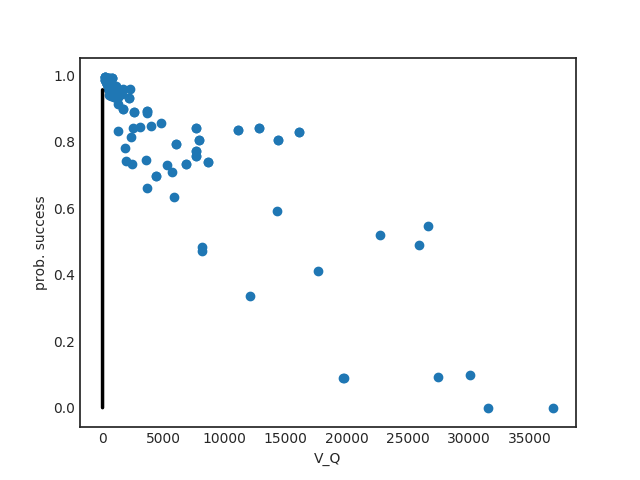
\includegraphics[width=0.75\linewidth]{ps_q_3000_0_005} 
    \caption{Quantum Volume} 
    \label{fig:ps_q_3000} 
  \end{subfigure} 
  \caption{Plotting probability of success against number of gates, swaps, depth and Quantum Volume}
  \label{fig:ps_3000} 
\end{figure}




\subsubsection{Two-qubit gates}
\label{sec:org55a4e81}

$$\rho _{f',Y} = 0.5784$$

\begin{figure}[htbp]
\centering
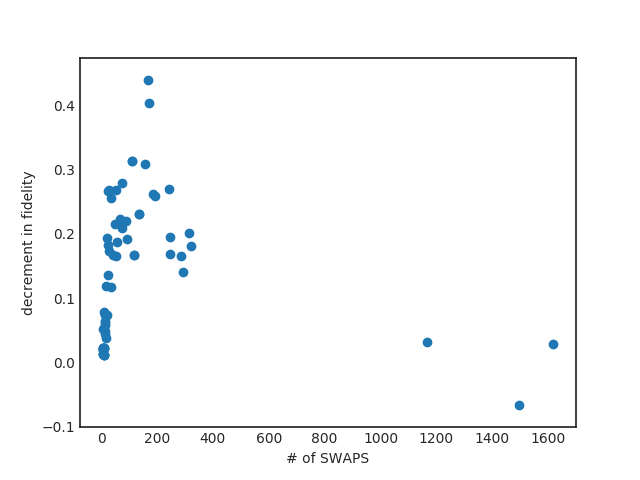
\includegraphics[width=0.7\textwidth]{f_s_2qg_3000.png}
\caption{\label{fig:orgb613639}
Number of swaps and fidelity difference relationship's}
\end{figure}

\subsection{\(t_1=1000\)}
\label{sec:orge90e504}

\begin{center}
\captionof{table}{\label{tab:org9cf67c7}
Pearson correlation coefficient for decoherence time of \(t_1 = 1000\) and measurement error 0f 0.005}
\begin{tabular}{lrrrr}
 & \# of Gates & \# of SWAPs & Depth & \(V_Q\)\\
\hline
\(\rho _{f,Y}\) & -0.7637 & -0.6658 & -0.7354 & -0.7029\\
\(\rho _{p_s,Y}\) & -0.8341 & -0.7484 & -0.8076 & -0.7686\\
\hline
\end{tabular}
\end{center}


\begin{figure}[H] 
  \begin{subfigure}[b]{0.5\linewidth}
    \centering
    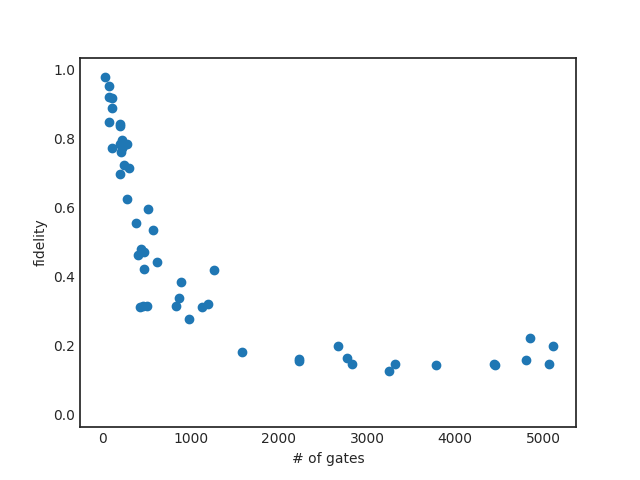
\includegraphics[width=0.75\linewidth]{f_g_1000_0_005} 
    \caption{Number of gates} 
    \label{fig:f_g_1000} 
    \vspace{4ex}
  \end{subfigure}%% 
  \begin{subfigure}[b]{0.5\linewidth}
    \centering
    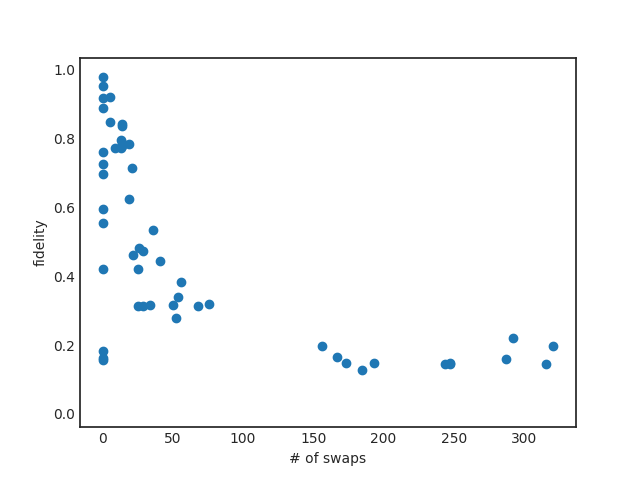
\includegraphics[width=0.75\linewidth]{f_s_1000_0_005} 
    \caption{Number of SWAPs} 
    \label{fig:f_s_1000} 
    \vspace{4ex}
  \end{subfigure} 
  \begin{subfigure}[b]{0.5\linewidth}
    \centering
    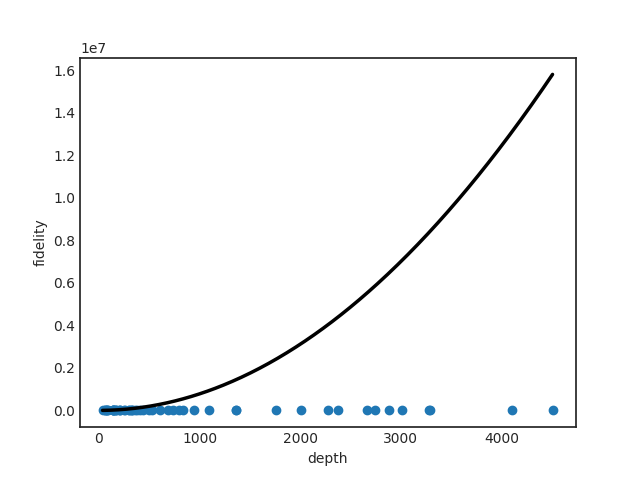
\includegraphics[width=0.75\linewidth]{f_d_1000_0_005} 
    \caption{Depth} 
    \label{fig:f_d_1000} 
  \end{subfigure}%%
  \begin{subfigure}[b]{0.5\linewidth}
    \centering
    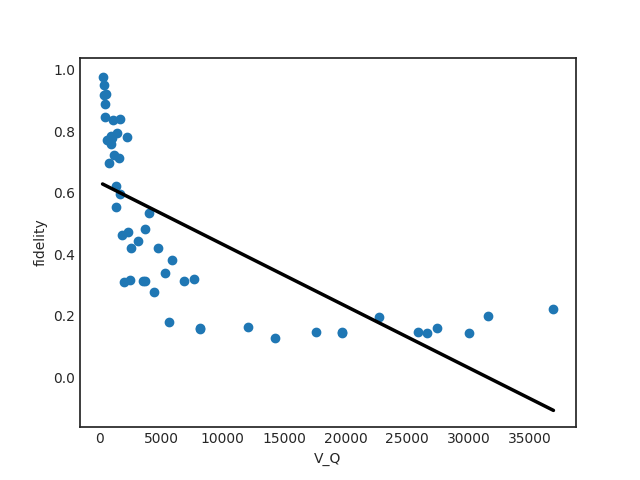
\includegraphics[width=0.75\linewidth]{f_q_1000_0_005} 
    \caption{Quantum Volume} 
    \label{fig:f_q_1000} 
  \end{subfigure} 
  \caption{Plotting fidelity against number of gates, swaps, depth and Quantum Volume}
  \label{fig:f_1000} 
\end{figure}

\begin{figure}[H] 
  \begin{subfigure}[b]{0.5\linewidth}
    \centering
    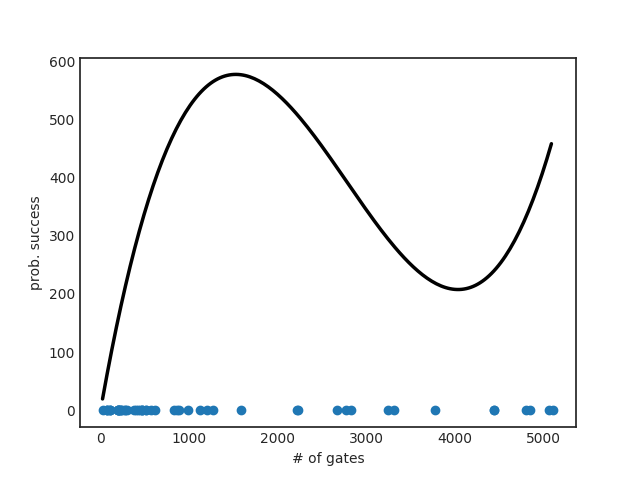
\includegraphics[width=0.75\linewidth]{ps_g_1000_0_005} 
    \caption{Number of gates} 
    \label{fig:ps_g_1000} 
    \vspace{4ex}
  \end{subfigure}%% 
  \begin{subfigure}[b]{0.5\linewidth}
    \centering
    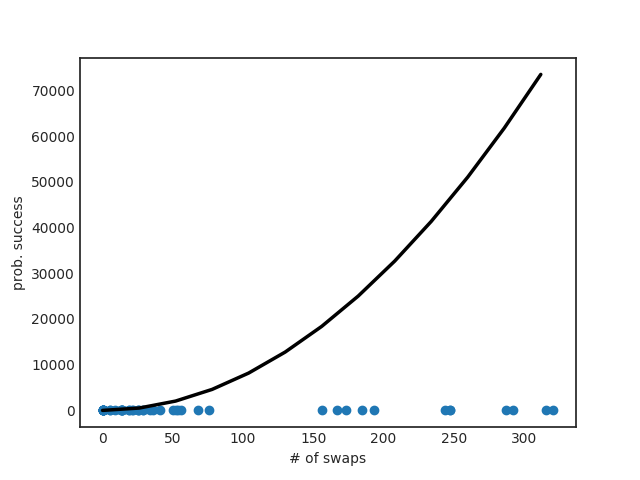
\includegraphics[width=0.75\linewidth]{ps_s_1000_0_005} 
    \caption{Number of SWAPs} 
    \label{fig:ps_s_1000} 
    \vspace{4ex}
  \end{subfigure} 
  \begin{subfigure}[b]{0.5\linewidth}
    \centering
    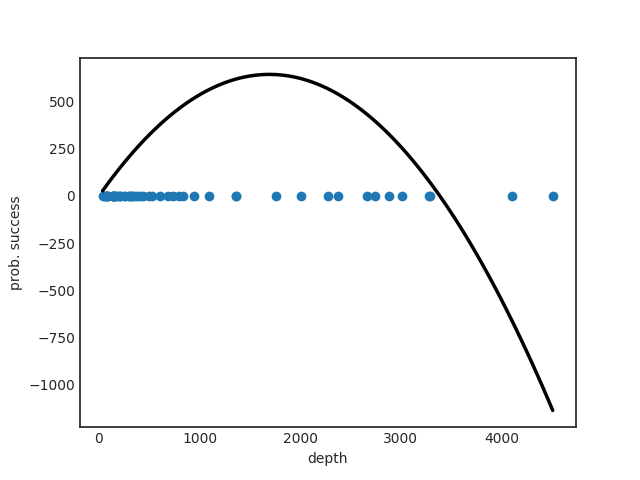
\includegraphics[width=0.75\linewidth]{ps_d_1000_0_005} 
    \caption{Depth} 
    \label{fig:ps_d_1000} 
  \end{subfigure}%%
  \begin{subfigure}[b]{0.5\linewidth}
    \centering
    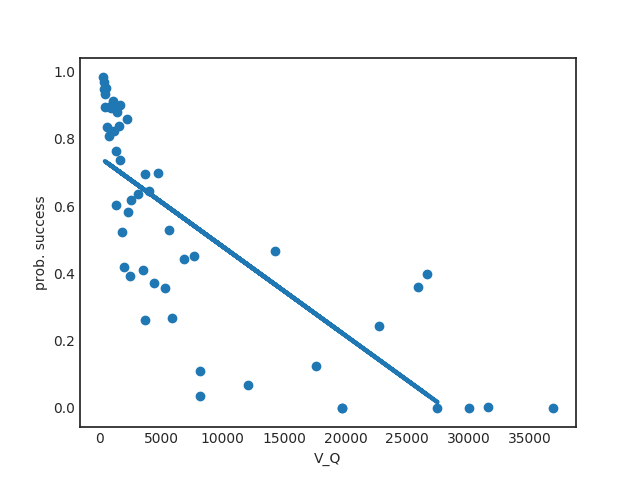
\includegraphics[width=0.75\linewidth]{ps_q_1000_0_005} 
    \caption{Quantum Volume} 
    \label{fig:ps_q_1000} 
  \end{subfigure} 
  \caption{Plotting probability of success against number of gates, swaps, depth and Quantum Volume}
  \label{fig:ps_1000} 
\end{figure}

\subsubsection{Two-qubit gates}
\label{sec:org58ff493}

$$\rho _{f',Y} = -0.639791579133524$$

\begin{figure}[htbp]
\centering
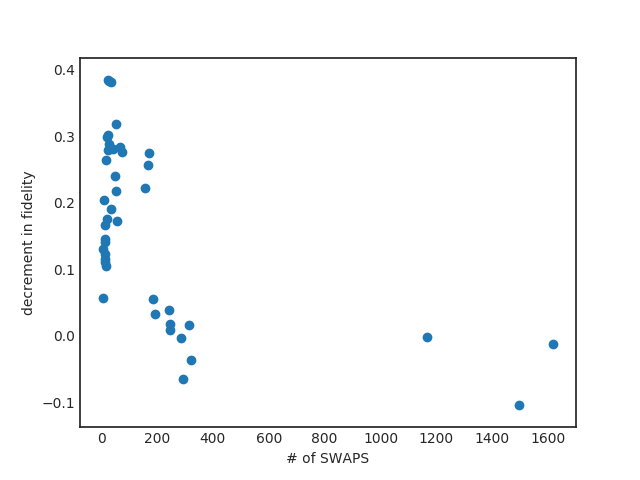
\includegraphics[width=0.7\textwidth]{f_s_2qg_1000.png}
\caption{\label{fig:org68efa8f}
Number of swaps and fidelity difference relationship's}
\end{figure}

\subsection{No measurement error and \(t_1=3000\)}
\label{sec:org4dac358}

\begin{center}
\captionof{table}{\label{tab:org4189d66}
Pearson correlation coefficient for decoherence time of \(t_1 = 3000\) and probability 0 for the measurement}
\begin{tabular}{lrrrr}
 & \# of Gates & \# of SWAPs & Depth & \(V_Q\)\\
\hline
\(\rho _{f,Y}\) & -0.9246 & -0.8482 & -0.9012 & -0.8697\\
\(\rho _{p_s,Y}\) & -0.9495 & -0.8972 & -0.9334 & -0.8985\\
\hline
\end{tabular}
\end{center}


\begin{figure}[H] 
  \begin{subfigure}[b]{0.5\linewidth}
    \centering
    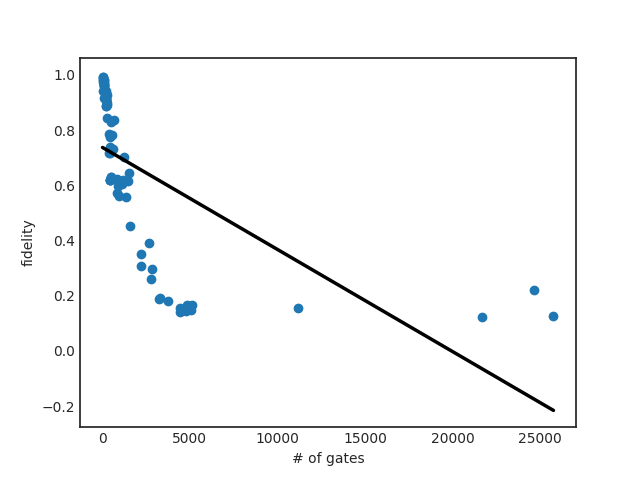
\includegraphics[width=0.75\linewidth]{f_g_3000_0} 
    \caption{Number of gates} 
    \label{fig:f_g_3000_0} 
    \vspace{4ex}
  \end{subfigure}%% 
  \begin{subfigure}[b]{0.5\linewidth}
    \centering
    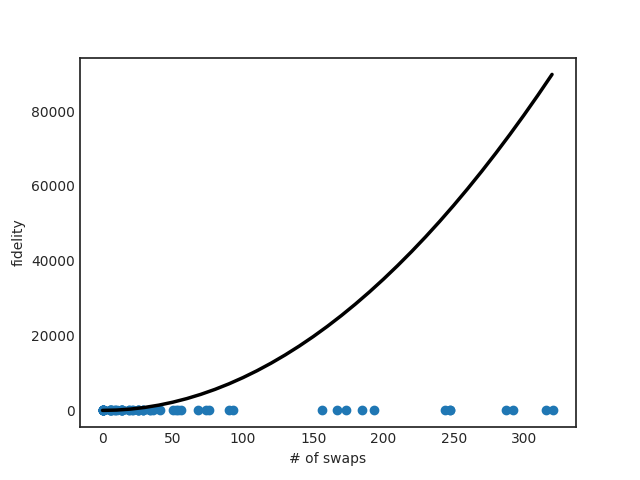
\includegraphics[width=0.75\linewidth]{f_s_3000_0} 
    \caption{Number of SWAPs} 
    \label{fig:f_s_3000_0} 
    \vspace{4ex}
  \end{subfigure} 
  \begin{subfigure}[b]{0.5\linewidth}
    \centering
    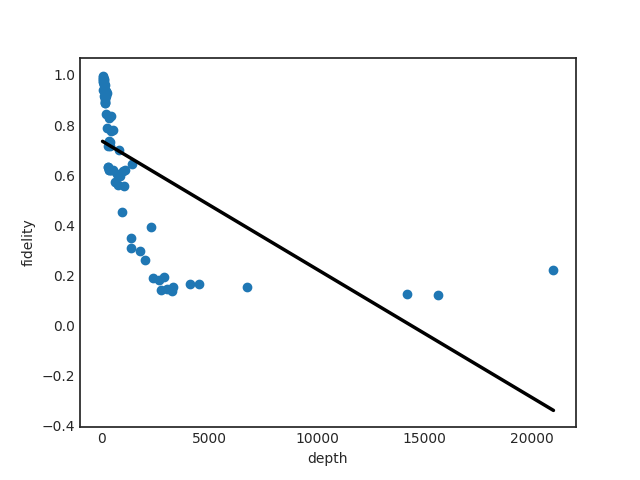
\includegraphics[width=0.75\linewidth]{f_d_3000_0} 
    \caption{Depth} 
    \label{fig:f_d_3000_0} 
  \end{subfigure}%%
  \begin{subfigure}[b]{0.5\linewidth}
    \centering
    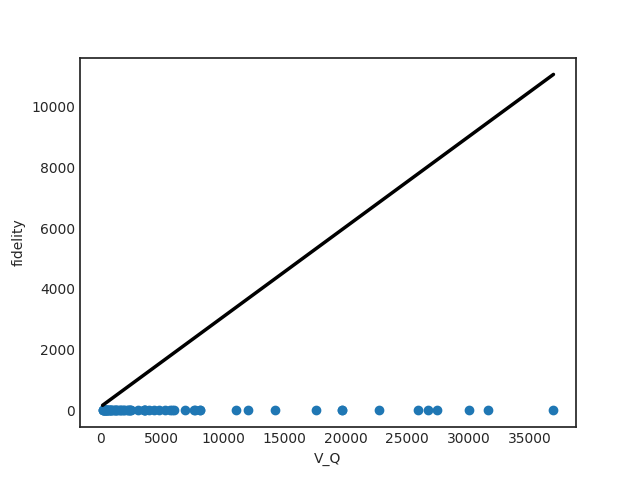
\includegraphics[width=0.75\linewidth]{f_q_3000_0} 
    \caption{Quantum Volume} 
    \label{fig:f_q_3000_0} 
  \end{subfigure} 
  \caption{Plotting fidelity against number of gates, swaps, depth and Quantum Volume}
  \label{fig:f_3000_0} 
\end{figure}

\begin{figure}[H] 
  \begin{subfigure}[b]{0.5\linewidth}
    \centering
    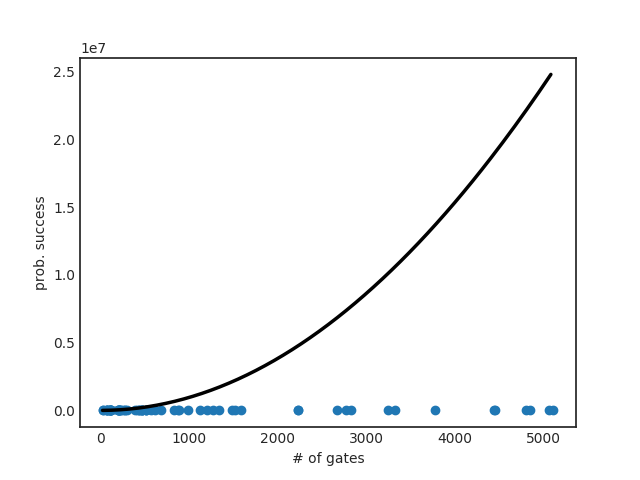
\includegraphics[width=0.75\linewidth]{ps_g_3000_0} 
    \caption{Number of gates} 
    \label{fig:ps_g_3000_0} 
    \vspace{4ex}
  \end{subfigure}%% 
  \begin{subfigure}[b]{0.5\linewidth}
    \centering
    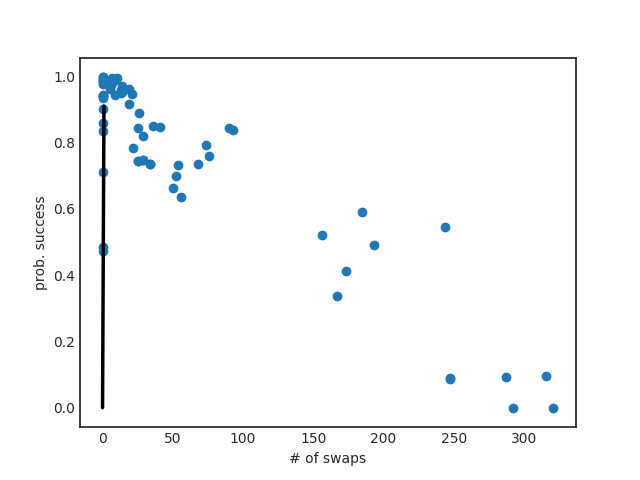
\includegraphics[width=0.75\linewidth]{ps_s_3000_0} 
    \caption{Number of SWAPs} 
    \label{fig:ps_s_3000_0} 
    \vspace{4ex}
  \end{subfigure} 
  \begin{subfigure}[b]{0.5\linewidth}
    \centering
    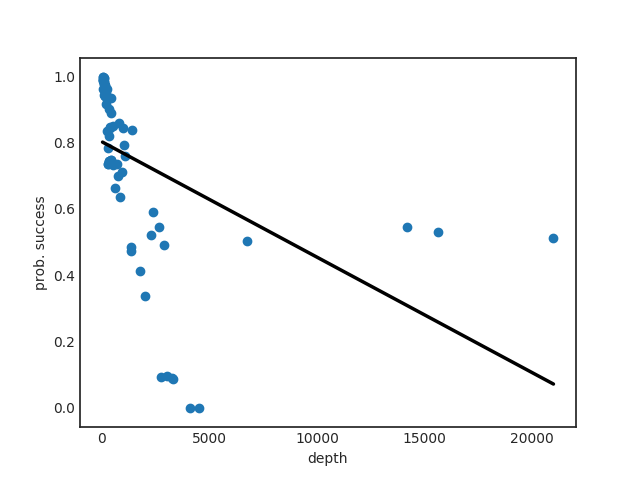
\includegraphics[width=0.75\linewidth]{ps_d_3000_0} 
    \caption{Depth} 
    \label{fig:ps_d_3000_0} 
  \end{subfigure}%%
  \begin{subfigure}[b]{0.5\linewidth}
    \centering
    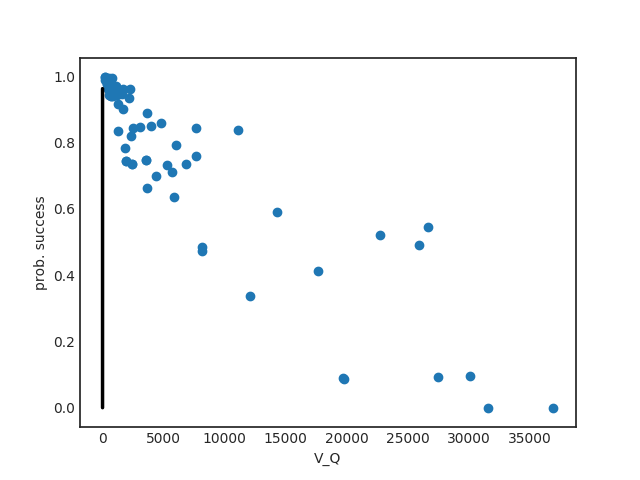
\includegraphics[width=0.75\linewidth]{ps_q_3000_0} 
    \caption{Quantum Volume} 
    \label{fig:ps_q_3000_0} 
  \end{subfigure} 
  \caption{Plotting probability of success against number of gates, swaps, depth and Quantum Volume}
  \label{fig:ps_3000_0} 
\end{figure}

\subsubsection{Two-qubit gates}
\label{sec:orgb7206a2}

$$\rho _{f',Y} = 0.4445$$

\begin{figure}[htbp]
\centering
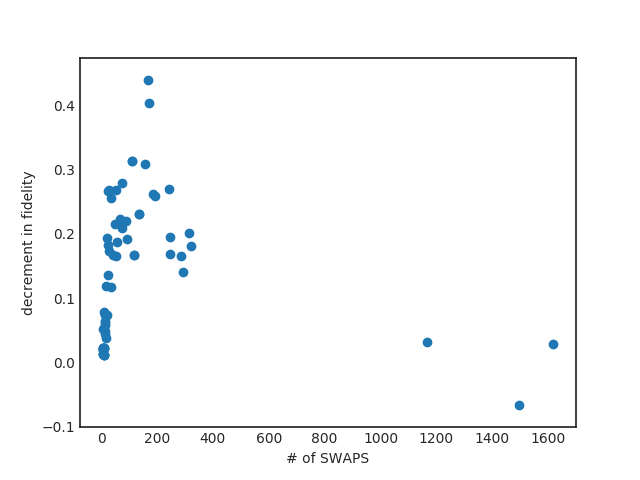
\includegraphics[width=0.7\textwidth]{f_s_2qg_3000.png}
\caption{\label{fig:org36a432c}
Number of swaps and fidelity difference relationship's}
\end{figure}
\end{document}
